\documentclass[12pt,letterpaper]{article}
\usepackage[utf8]{inputenc}
\usepackage{amsmath}
\usepackage{amsfonts}
\usepackage{amssymb}
\usepackage{listings}
\usepackage{graphicx}
\usepackage{tikz}
\usepackage{pgfplots}
\usepackage{tcolorbox}
\usepackage{hyperref}
\usepackage{color}
\usepackage[left=2cm,right=2cm,top=2cm,bottom=2cm]{geometry}

\pgfplotsset{compat=1.13}
\graphicspath{ {images/} }

\author{Aaron Trent}
\title{Rendering Notes}

\newcommand{\iu}{{i\mkern1mu}}

\newenvironment{tight_enumerate}{
\begin{enumerate}
  \setlength{\itemsep}{0pt}
  \setlength{\parskip}{0pt}
}{\end{enumerate}}

\setcounter{secnumdepth}{3}

\makeatletter
\begin{document}

\maketitle

\begin{center}
Collection of equations and algorithms for use in the Combustion Engine, 
as well as general reference for developers wishing to understand the final equations and how I came to them.
\end{center}

{\footnotesize \tableofcontents}

\setlength{\parindent}{4em}
\setlength{\parskip}{0.8em}

\newpage

\part{Theory}

\section{Physically Based Rendering (PBR)}

Physically Based Rendering (or Physically Based Shading) is simply the technique of using real-world-like parameters to represent
a material, for example \textbf{Roughness}, \textbf{Anisotropy}, \textbf{Metalness}, \textbf{Index of Refraction} ($\eta$), and so forth.

\subsection{Physical Correctness}

By itself, PBR does not guarantee a realistic image. The equations and algorithms used to render the image must be physically correct.
That is, they must obey the laws of physics to properly simulate light.

\section{Microfacet Theory}

Microfacet theory describes the surface of an object as being composed of incredibly tiny mirrors called microfacets. 
The microfacets are oriented in different directions based on surface roughness. The more smooth the surface, the more mirrors line up with the surface normal,
forming a more mirrored macroscopic surface. Rougher surfaces are equivalent to the microfacets being oriented in ever more random directions,
up until a point of entirely rough surfaces where the microfacets are totally randomly oriented and 
scatter light in all directions.

Since microfacets themselves are less intuitive, they are usually abstracted to become microgeometry, 
which is the microscopic ridges and crevices of a surface, where roughness and smoothness are as we know them traditionally.

At this abstraction level, it makes more sense that rougher surfaces are blurrier, while smoother surfaces are shinier.

\newpage

\section{Fresnel Effect}

\textit{"Everything has Fresnel!" - Internet}

If you haven't heard this before, you have now. Everything has Fresnel. However, what is Fresnel?

Put simply, the Fresnel effect determines how much light is reflected off of or transmitted into a surface. 
Reflected light forms specular highlights, while transmitted light becomes diffuse reflections or subsurface scattering.

For transparent materials, like glass, transmitted light is also refracted and passes all the way through it.

The Fresnel effect is governed by three primary variables (excluding any vectors):

\begin{tight_enumerate}
    \item The Internal Index of Refraction ($\eta_i$)
    \item The Extinction Coefficient ($k$)
    \item The External Index of Refraction ($\eta_o$)
\end{tight_enumerate}

where the internal IOR ($\eta_i$) is the index of refraction of the material itself, 
the extinction coefficient ($k$) is effectively how conductive the material is, and the external IOR ($\eta_o$) is the 
index of refraction of the material the object is contained in. 

Normally, the external IOR is approximately 1.0, because the IOR of Air is approximately 1.0, 
so many forms of the Fresnel equations simply omit it.

However, if you wish to render an object as it appears underwater, the external IOR must be set to approximately 1.33 (the IOR of Water), 
or it will appear incorrect.

For metals, the interal IOR and extinction coefficient form a complex IOR in the form:
$$\eta + \iu k$$
where the color of the metal can be derived from it's wavelength-specific IORs.

\newpage

\section{Wavelength Response}

\subsection{Computer Color}

Color in computer graphics is primarily RGB. Despite HSV/HSL/YUV/etc. color representations, RGB remains the primary way to 
represent color in computers. The reason for this is that the human eye only perceives Red, Green and Blue colors for its three cone type.
The science of human color perception is quite in-depth and not necessary here, but the gist of it is that humans see a range of wavelengths
for each primary color, with perception strength in roughly Gaussian curve shapes.

\subsection{RGB Wavelengths and Human Eyesight}

Here are the wavelengths used in Combustion:
\begin{align*}
    \text{Red}   &= 620\text{nm} - 740\text{nm}\\
    \text{Green} &= 495\text{nm} - 570\text{nm}\\
    \text{Blue}  &= 450\text{nm} - 495\text{nm}\\
\end{align*}

where the human eye's response to individual wavelengths is this:
\begin{figure}[htbp]
    \centering
    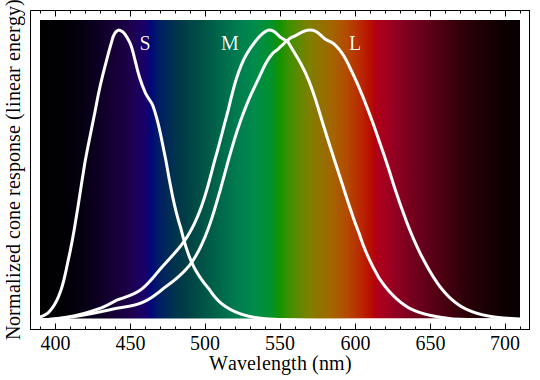
\includegraphics[width=20em]{Cone-fundamentals-with-srgb-spectrum}
    \caption{Human Eye Wavelength Response}
    \label{fig:eye_wavelength_response}
\end{figure}

which can be approximated using a modified Gaussian function like this:
\begin{center}
	\pgfplotsset{width=15em}
	\begin{tikzpicture}
		\begin{axis}[
		    legend pos=south east,
		    axis lines = left,
		    xlabel = $x$,
		    ylabel = {$f(x)$},
		    clip = false,
		]
		\addplot [
		    domain=-1.5:2.5,
		    samples=50,
		    color=black,
		]
		{e^(-(x - (1/2))^2)};
		\addlegendentry{$e^{-{\left( x - \frac{1}{2} \right)}^2}$}
		%\draw (axis cs:0.5,0) -- (axis cs:0.5,1) node [above]{$f(0.5) = 1$};
		\end{axis}
	\end{tikzpicture}
\end{center}

to form:

\begin{figure}[htbp]
    \centering
	\pgfplotsset{width=30em, height=15em}
	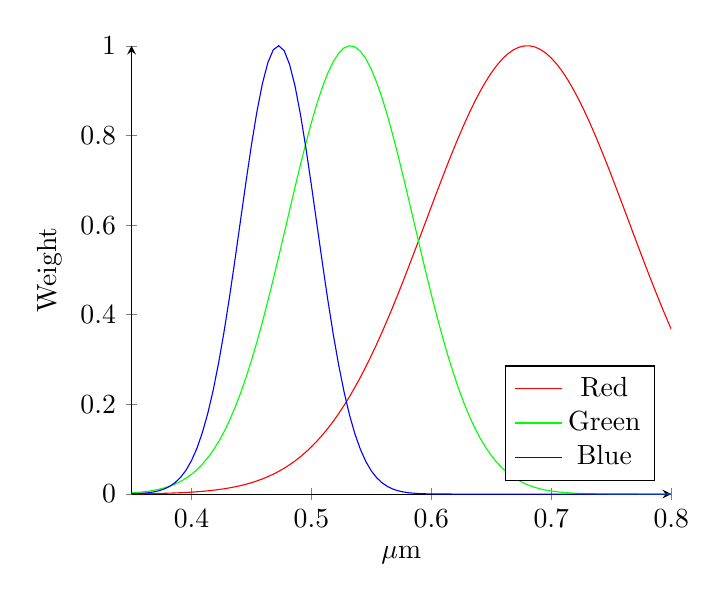
\begin{tikzpicture}
		\begin{axis}[
		    legend pos=south east,
		    axis lines = left,
		    xlabel = $\mu\text{m}$,
		    ylabel = {Weight},
		]
		\addplot [
		    domain=0.35:0.8,
		    samples=100,
		    color=red,
		]
		{e^-(((((x-0.62)/(0.74-0.62)) - (1/2)))^2)};
		\addlegendentry{Red}
	    \addplot [
		    domain=0.35:0.8,
		    samples=100,
		    color=green,
		]
		{e^-(((((x-0.495)/(0.57-0.495)) - (1/2)))^2)};
		\addlegendentry{Green}
		\addplot [
		    domain=0.35:0.8,
		    samples=100,
		    color=blue,
		]
		{e^-(((((x-0.45)/(0.495-0.45)) - (1/2)))^2)};
		\addlegendentry{Blue}
		\end{axis}
	\end{tikzpicture}
	\caption{Weighted RGB Wavelength Response}
	\label{fig:rgb_wavelength_response}
\end{figure}
which is similar to our perception of pure Red, Green and Blue. Note that they don't line up exactly, 
because there is a difference between wavelength and RGB color.

So by using this simple form to our advantage, we can perform a weighted average of 
any wavelength dependent optical properties like so:

$$
V = \frac{\int_{w_{min}}^{w_{max}}{f\left(x\right)p\left(x\right)dx}}
     {\left( w_{max} - w_{min} \right) \int_{w_{min}}^{w_{max}}{p\left(x\right)dx}}
$$
where $p(x)$ is:
$$
p(x) = e^{-{\left( \frac{x-w_{min}}{w_{max}-w_{min}} - \frac{1}{2} \right)}^2}
$$
or the original distribution scaled to the wavelength range like so:
$$
p(\frac{x-w_{min}}{w_{max}-w_{min}}) = e^{-{\left( x - \frac{1}{2} \right)}^2}
$$

\newpage

\part{Light Equations}

\section{Specular Reflectance}

\subsection{Cook-Torrance}

The Cook-Torrance equation is the core component for specular reflections today.

\begin{tcolorbox}[colback=white]
    Variables for equations:
    \\
    \rule{2in}{0.4pt}
	\begin{flalign*}
		N &= \text{unit surface normal}&\\
		V &= \text{view vector}\\
		L &= \text{light vector}\\
		H &= \frac{V + L}{\lVert V + L \rVert} = \text{halfway vector and microfacet normal}\\
		\eta &= \text{Index of Refraction}\\
		\alpha &= \text{surface roughness}
	\end{flalign*}
\end{tcolorbox}

It should be noted that these are ONLY specular reflections. That is, light which is reflected without diffusing into the material surface.
For diffuse materials and how to mix diffuse and specular reflections, keep reading.

\newpage

\subsubsection{R. Cook and K. Torrance 1981}

Original Definition:

$$
f_{spec} = \frac{D F G}{\pi \left( \omega_o \cdot n \right) \left( \omega_i \cdot n \right) }
$$
where $\omega_o$ is the view direction and $\omega_i$ is the incoming light direction.

$G$, the \textbf{Geometric Attenuation} function, which describes self-shadowing due to microfacet orientation and roughness, is defined as:
$$
G_{Cook-Torrance} = min \left\lbrace1, 
              \frac{2 \left( N \cdot H \right) \left( N \cdot V \right)}{\left( V \cdot H \right)}, 
              \frac{2 \left( N \cdot H \right) \left( N \cdot L \right)}{\left( V \cdot H \right)}
        \right\rbrace
$$

$D$, the \textbf{Microfacet Distribution} function, is the Beckmann distribution,\\
which is defined as:
$$
D_{Beckmann} = \frac{
    \text{exp}\left(
                    \frac{{\left( n \cdot m \right)}^2 - 1}
                         {\alpha^2 {\left( n \cdot m \right)}^2} \right)}
    {\pi \alpha^2 {\left( n \cdot m \right)}^4}
$$
where $\alpha$ is the surface roughness from $\left[0,1\right]$, but it has been simplified to:

$F$ is the \textbf{Fresnel} term, which was originally defined as:
$$
F = \frac{1}{2}\frac{{\left( g - c \right)}^2}{{\left( g + c \right)}^2} 
    \left\lbrace
        1 + \frac{
            {\left[c\left( g + c \right) - 1\right]}^2
                }{
            {\left[c\left( g - c \right) + 1\right]}^2
                }
    \right\rbrace
$$
where
\begin{flalign*}
c &= \cos\theta = V \cdot H&\\
g^2 &= \eta^2 + c^2 - 1\\
\eta &= \frac{1 + \sqrt{F_0}}{1 - \sqrt{F_0}}
\end{flalign*}
and $F_0$ is defined as:
\begin{align*}
F_0 &= {\left\lbrace \frac{\eta - 1}{\eta + 1} \right\rbrace}^2
\end{align*}
where $\eta$ is the Index of Refraction of the material. Depending on how you do things, $F_0$ can be avoided entirely by just using the raw IOR $\eta$.

\newpage

\subsubsection{Walter 2007 (GGX)}

Walter 2007 updates the Cook-Torrance model with a better set of equations that are commonly referred to as GGX.

GGX Cook-Torrance form:

$$
f_{spec} = \frac{D F G}{4 \left( \omega_o \cdot n \right) \left( \omega_i \cdot n \right) }
$$
where $G$ is split into two functions like so:
$$G = G_l(\omega_i) G_l(\omega_o)$$

Here, the Geometric Attenuation term is broken into two functions, collectively referred to as the Smith shadow-masking function. Each partial geometric attenuation function is the same, but is passed separate vector for light and view directions, then multiplied together.

Also note the replacement of $\pi$ with just $4$. I often see these used interchangeably around the internet, but they should remain distinct depending on how it is used. GGX works better with $4$.

For the GGX equations, $G_l$ is defined as:
$$
G_l(v) = \chi^+ \left(\frac{\omega_v \cdot \omega_g}{\omega_v \cdot \omega_m} \right)
\frac{2}{1 + \sqrt{1 + \alpha^2 \tan^2\theta_v}}
$$
where $\omega_v$ is the view direction, $\omega_g$ is the unit surface normal, $\omega_m$ is the halfway vector, and $\omega_v$ is the incoming or outgoing direction.

The GGX Distribution function ($D$) is defined as:
$$
D = \chi^+\left(n \cdot m\right) \frac{\alpha^2}{\pi \cos^4\theta {\left(  \alpha^2 + \tan^2\theta \right)}^2}
$$
or simplified to:
$$
D = \chi^+\left(n \cdot m\right) \frac{\alpha^2}{\pi {\left( {\left( n \cdot m \right)}^2 \left(\alpha^2 - 1\right) + 1 \right)}^2}
$$
with an anisotropic form defined as:
$$
D = \chi^+\left(n \cdot m\right) \frac{1}{\pi \alpha_x \alpha_y} \frac{1}{{\left(
    \frac{{\left( x \cdot m \right)}^2}{\alpha^{2}_{x}} +
    \frac{{\left( y \cdot m \right)}^2}{\alpha^{2}_{y}} +
    {\left( n \cdot m \right)}^2
\right)}^2}
$$
as you can see, it takes two $\alpha$ (roughness) values and two anisotropy direction values ($x$ and $y$) to control anisotropy.

\newpage

\section{Diffuse Reflectance}

What light isn't directly reflected in the form of specular highlights is transmitted into the surface. However, most surfaces simply scatter the light 
below the surface and re-emit it in the form of colored diffuse light.

\subsection{Lambertian Diffuse Model}

For perfectly smooth surfaces, diffuse reflectance can be approximated by a single operation:

$$
f_{diffuse} = N \cdot L
$$
which is simply $\cos\theta$ between the light and normal vectors, which has a curve like this:
\begin{figure}[htbp]
  \begin{minipage}[t]{0.5\linewidth}
    \centering
    \pgfplotsset{width=15em}
	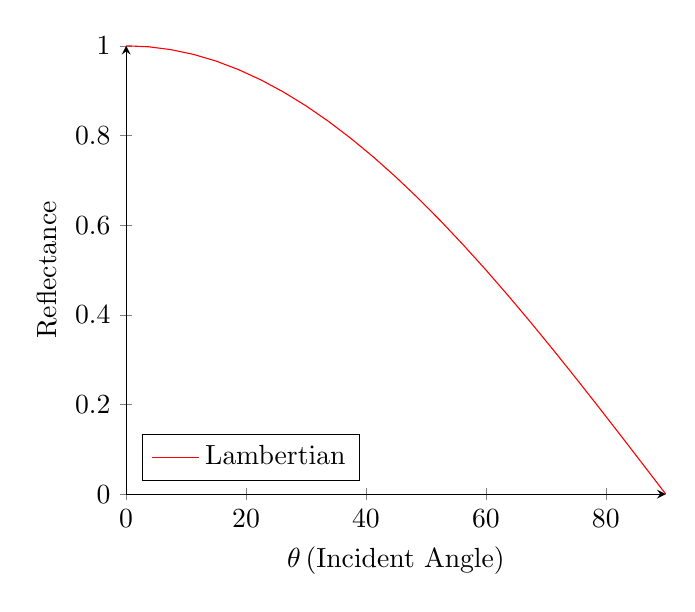
\begin{tikzpicture}
		\begin{axis}[
		    legend pos=south west,
		    axis lines = left,
		    xlabel = $\theta \left(\text{Incident Angle}\right)$,
		    ylabel = {Reflectance},
		]
		\addplot [
		    domain=0:90,
		    samples=25,
		    color=red,
		]{cos(x)};
		\addlegendentry{Lambertian}
		\end{axis}
	\end{tikzpicture}
    \caption{Lambertian reflectance}
  \end{minipage}
  \hspace{-16pt}
  \begin{minipage}[t]{0.5\linewidth}
    \centering
	\pgfplotsset{width=20em}
	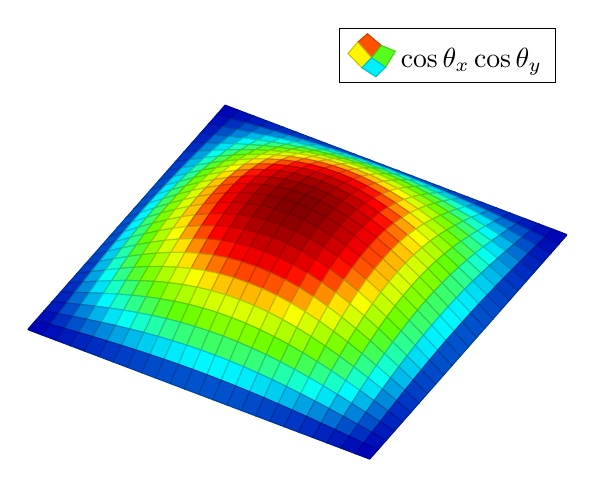
\begin{tikzpicture}
		\begin{axis}[
		    hide axis,
		    colormap/bluered,
		    view={30}{70}
		]
		\addplot3[
		    surf,
		    samples=25,
		    domain=-90:90,
		]
		{cos(x)*cos(y)};
		\addlegendentry{$\cos\theta_x \cos\theta_y$}
		\end{axis}
	\end{tikzpicture}
    \caption{3D plot}
  \end{minipage}
\end{figure}

Lambertian is the most commonly used diffuse model mostly because of its simplicity. 
It's usually computed anyway for the specular component, so it's effectively free.

However, it does not account for surface roughness, so things get kind of weird looking in PBR heavy workflows.

You can see this effect more in Figure {\color{blue}\ref{fig:lambert_orennayar_comparison}} on the next page.

\newpage

\subsection{Oren-Nayar Diffuse Model}

Oren-Nayar is a "newer" (1994) set of equations based on empirical data that more accurately simulates surfaces of varying roughness.

\begin{figure}[htbp]
    \centering
    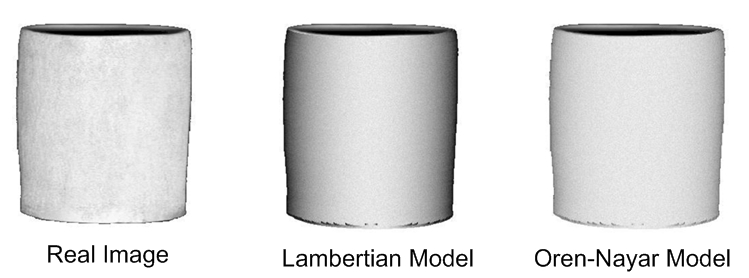
\includegraphics[width=20em]{Oren-nayar-vase2}
    \caption{Comparison of Lambertian and Oren-Nayar models}
    \label{fig:lambert_orennayar_comparison}
\end{figure}

As you can see, Oren-Nayar does a much better job than traditional Lambertian diffuse. 
It more accurately simulates rough surfaces, and is therefore much more useful in modern PBR workflows.

The full form of the Oren-Nayar equation is defined as:

$$
L_{r}={\frac{\rho}{\pi}}\cdot \cos\theta_{i} \cdot (A + (B \cdot \max[0, \cos(\phi_i - \phi_r)] \cdot \sin \alpha \cdot \tan \beta )) \cdot E_{0}
$$
where
\begin{flalign*}
A &= 1 - 0.5{\frac{\sigma^{2}}{\sigma^{2} + 0.57}}&\\
B &= 0.45 {\frac{\sigma^{2}}{\sigma^{2} + 0.09}}\\
\alpha &= \max(\theta_{i}, \theta_{r})\\
\beta &= \min(\theta_{i}, \theta_{r})
\end{flalign*}
and $\rho$ is the surface albedo (diffuse absorption), $\sigma$ is the surface roughness, and $\phi_i$ and $\phi_r$ are the azimuth angles
\begin{figure}[htbp]
    \begin{minipage}[t]{0.5\linewidth}
        \centering
        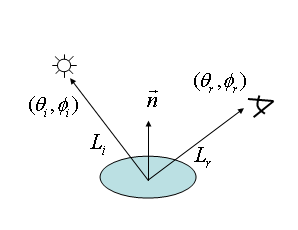
\includegraphics[width=15em]{Oren-nayar-reflection}
        \caption{Reflectance Diagram}
    \end{minipage}
    \hspace{-6pt}
    \begin{minipage}[t]{0.5\linewidth}
        \centering
        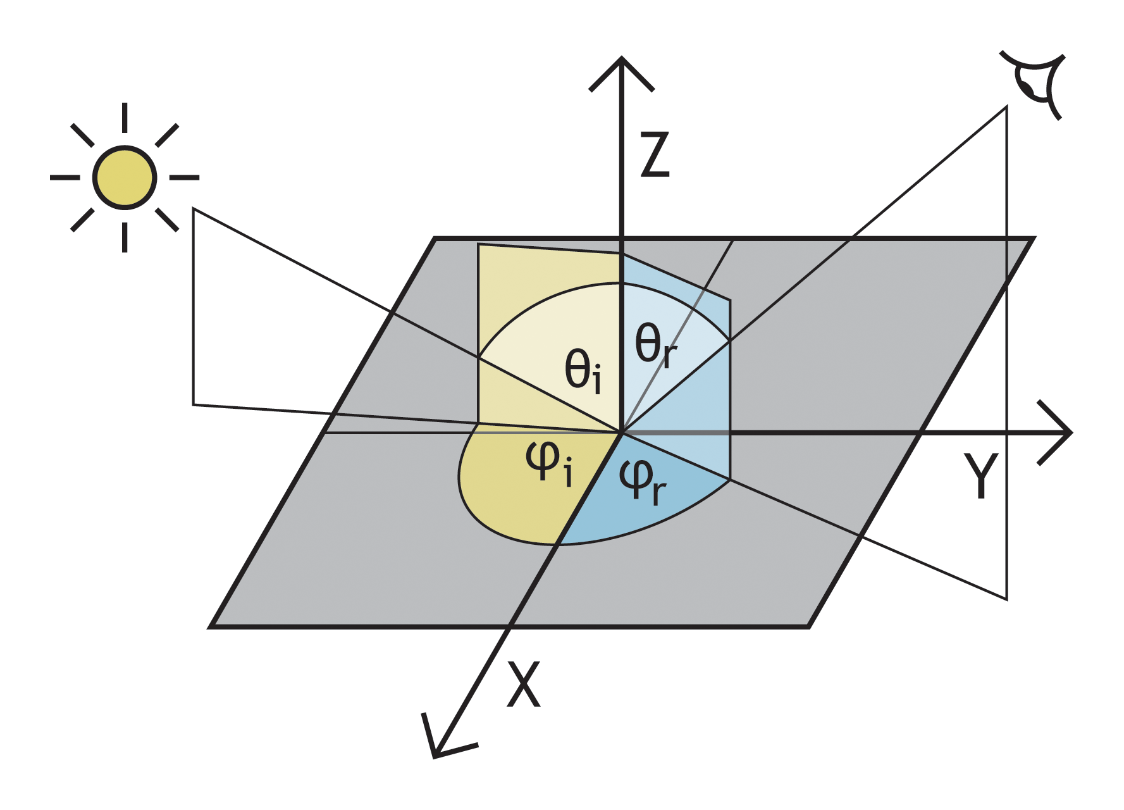
\includegraphics[width=15em]{Angle_overview}
        \caption{Angle Diagram}
    \end{minipage}    
\end{figure}

\newpage

\section{Fresnel Equations}

The Fresnel equations determine how much light is reflected off of a surface, versus how much light is transmitted into it. Therefore,
they are critical for correctly rendering any realistic material.

\noindent Most of these equations were taken from 
{\color{blue}\href{https://seblagarde.wordpress.com/2013/04/29/memo-on-fresnel-equations/}{Memo on Fresnel equations by Sébastien Lagarde}}

The full Dielectric-Conductor Fresnel equations are as follows:

\begin{align*}
    a^2 &= \frac{1}{2\eta_i^2}\left(\sqrt{{\left(\eta_t^2 - k_t^2 - \eta_i^2 \sin^2\theta\right)}^2 + 4\eta_t^2 k_t^2} + \eta_t^2 - k_t^2 - \eta_i^2 \sin^2\theta\right)\\
    b^2 &= \frac{1}{2\eta_i^2}\left(\sqrt{{\left(\eta_t^2 - k_t^2 - \eta_i^2 \sin^2\theta\right)}^2 + 4\eta_t^2 k_t^2} - \eta_t^2 + k_t^2 + \eta_i^2 \sin^2\theta\right)\\
    R_s &= \frac{a^2 + b^2 - 2a \cos\theta + \cos^2\theta }{a^2 + b^2 + 2a \cos\theta + \cos^2\theta}\\
    R_p &= R_s \frac{a^2 + b^2 - 2a \sin\theta \tan\theta + \sin^2\theta \tan^2\theta}{a^2+b^2+2 a\sin\theta \tan\theta + \sin^2\theta \tan^2\theta}\\
\end{align*}
where
\begin{align*}
    \eta_t &= \text{Surface IOR ($t$ for transmitted)}\\
    k_t    &= \text{Surface Extinction Coefficient}\\
    \eta_i &= \text{External IOR ($i$ for incoming)}
\end{align*}

Furthermore, this gives us two reflectance values, $R_s$ and $R_p$, for parallel and perpendicular polarization of light.
If light polarization is not important, these can be average together into a single reflectance value like so:
$$
R = \frac{R_s + R_p}{2}
$$
or if polarization is important, these values should be linearly interpolated like so:
$$
R = \left(1 - \omega_t\right) R_s + \omega_t R_p
$$
where $\omega_t$ is the polarity weight in the domain $\left[0,1\right]$, so that $0$ is fully perpendicular polarized light, 
and $1$ is fully parallel polarized light. A weight of $\frac{1}{2}$ is equal to the first form 
where they are averaged together.

As mentioned in the Fresnel Effect theory section, the external IOR plays a very important role for scene that are not in air or vacuum. In air and/or vacuum, 
the external IOR is usually assumed to be 1 so the equation can be simplified, but for underwater scenes or something more exotic this parameter is absolutely necessary.

\newpage

\subsection{Metals}

Metals are unique because they have no diffuse reflections, 
and therefore their entire color is derived from the Fresnel effect on varying wavelengths of light.

As you can see below in Figures \ref{fig:gold_eta_t} and \ref{fig:gold_k_t}, 
Gold behaves very differently depending on wavelength. It absorbs blue-ish light and reflects more red-ish light, producing
its characteristic yellow color.

\begin{figure}[htbp]
    \begin{minipage}[t]{0.5\linewidth}
        \centering
		\begin{tikzpicture}
		    \begin{axis}[
		        xlabel = $\mu\text{m}$,
		        ylabel = $\eta_t$
		    ]
		        \addplot [mark=none, color=red] coordinates {
				    (0.43678, 1.44930)
					(0.44390, 1.41260)
					(0.45114, 1.36610)
					(0.45850, 1.30950)
					(0.46598, 1.24270)
					(0.47358, 1.16640)
					(0.48130, 1.08210)
					(0.48915, 0.99182)
					(0.49712, 0.89849)
					(0.50523, 0.80543)
					(0.51347, 0.71590)
					(0.52184, 0.63260)
					(0.53035, 0.55731)
					(0.53900, 0.49085)
					(0.54779, 0.43326)
					(0.55672, 0.38405)
					(0.56580, 0.34242)
					(0.57503, 0.30751)
					(0.58440, 0.27843)
					(0.59393, 0.25437)
					(0.60362, 0.23457)
					(0.61346, 0.21841)
					(0.62346, 0.20533)
					(0.63363, 0.19487)
					(0.64396, 0.18664)
					(0.65446, 0.18030)
					(0.66514, 0.17558)
					(0.67598, 0.17227)
					(0.68701, 0.17016)
					(0.69821, 0.16911)
					(0.70959, 0.16897)
					(0.72117, 0.16966)
					(0.73292, 0.17107)
		        };
		    \end{axis}
		\end{tikzpicture}
        \caption{Gold $\eta_t$}
        \label{fig:gold_eta_t}
    \end{minipage}
    \hspace{-6pt}
    \begin{minipage}[t]{0.5\linewidth}
        \centering
		\begin{tikzpicture}
		    \begin{axis}[
		        xlabel = $\mu\text{m}$,
		        ylabel = $k_t$
		    ]
		        \addplot [mark=none, color=blue] coordinates {
			        (0.43678, 1.79880)
					(0.44390, 1.78290)
					(0.45114, 1.76810)
					(0.45850, 1.75670)
					(0.46598, 1.75090)
					(0.47358, 1.75320)
					(0.48130, 1.76610)
					(0.48915, 1.79160)
					(0.49712, 1.83120)
					(0.50523, 1.88520)
					(0.51347, 1.95300)
					(0.52184, 2.03280)
					(0.53035, 2.12220)
					(0.53900, 2.21880)
					(0.54779, 2.32010)
					(0.55672, 2.42450)
					(0.56580, 2.53050)
					(0.57503, 2.63700)
					(0.58440, 2.74340)
					(0.59393, 2.84930)
					(0.60362, 2.95450)
					(0.61346, 3.05870)
					(0.62346, 3.16210)
					(0.63363, 3.26450)
					(0.64396, 3.36620)
					(0.65446, 3.46710)
					(0.66514, 3.56750)
					(0.67598, 3.66740)
					(0.68701, 3.76690)
					(0.69821, 3.86610)
					(0.70959, 3.96530)
					(0.72117, 4.06440)
					(0.73292, 4.16350)
			    };
		    \end{axis}
		\end{tikzpicture}
        \caption{Gold $k_t$}
        \label{fig:gold_k_t}
    \end{minipage}
\end{figure}

Consequently, because metals have different behaviors for different wavelengths of light, 
their color is created by the varying reflectance values at a given angle.

As you can see below in Figures \ref{fig:gold_reflectance} and \ref{fig:copper_reflectance}, 
Gold and Copper are given their unique colors by only the Fresnel effect, 
and reflecting more white light at greater grazing angle.

\begin{figure}[htbp]
  \begin{minipage}[t]{0.5\linewidth}
    \centering
	\begin{tikzpicture}
		\begin{axis}[
		    width=3in,
            ytick=\empty,
		    enlargelimits=false, 
		    axis equal=false, 
		    scale only axis,
		    axis equal image,
		    xtick={0,15,...,90},
		    xlabel = {Incident Angle in Degrees}]
 			\addplot graphics [xmin=0,xmax=90,ymin=0,ymax=20] {Gold-Reflectance};
		\end{axis}
	\end{tikzpicture}
	\caption{Gold}
	\label{fig:gold_reflectance}
  \end{minipage}
  \hspace{-6pt}
  \begin{minipage}[t]{0.5\linewidth}
    \centering
	\begin{tikzpicture}
		\begin{axis}[
		    width=3in,
            ytick=\empty,
		    enlargelimits=false, 
		    axis equal=false, 
		    scale only axis,
		    axis equal image,
		    xtick={0,15,...,90},
		    xlabel = {Incident Angle in Degrees}]
 			\addplot graphics [xmin=0,xmax=90,ymin=0,ymax=20] {Copper-Reflectance};
		\end{axis}
	\end{tikzpicture}
	\caption{Copper}
	\label{fig:copper_reflectance}
  \end{minipage}
\end{figure}

\newpage

\subsection{Dielectrics}

\begin{figure}[htbp]
    \centering
	\begin{tikzpicture}
		\begin{axis}[
		    enlargelimits=false, 
		    axis equal=false, 
		    scale only axis,
		    xtick={0,15,...,90},
		    xlabel = {Incident Angle in Degrees},
			ylabel = $\eta_t$]
			\addplot graphics [xmin=0,xmax=90,ymin=1,ymax=2] {Dielectric-Fresnel};
		\end{axis}
	\end{tikzpicture}
	\caption{Dielectric Fresnel Effect for various $\eta_t$}
	\label{fig:dielectric_fresnel}
\end{figure}

\end{document}
\makeatother